\section{Methodology}
\subsection{Network Generation}
\subsection{Infection Simulation}
To simulate the epidemic infection spread through the generated networks, we tested two different models: SIR and SIS.
\subsubsection{SIR}
The initials for this models stands for: Susceptible, Infected and Recovered. This simulate a disease that infects with probability $\mu_{SI}$, where this probability is dependent from how many contacts with infected hosts it is having. Basically, every node in susceptible state, can be infected by each connection with an infected host by a probability $\beta$. Then an infected host can recover with probability $\mu_{IR}$, where this probability is constant for all the nodes, in our case we set $\mu_{IR}=\gamma$. Finally when the host has ben recovered, it can't get infected again. So basically each host follows the state machine shown in figure \ref{fig:sir}.
\begin{figure}[htbp]
    \centering
    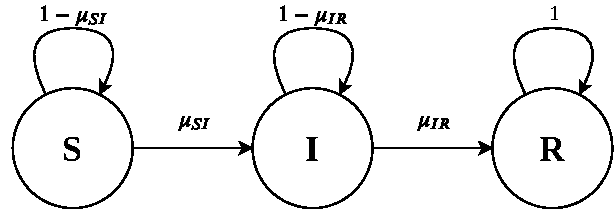
\includegraphics[width=\linewidth]{../img/SIR_model.pdf}
    \caption{SIR model representation.}
    \label{fig:sir}
\end{figure}

Assuming we have an adjacency list $W$, where each position is equal to the weight between the two nodes. In order to simulate this in an optimal way, at each time step, we go through all nodes of the network and do the following:
\begin{itemize}
    \item \textbf{If node i is Susceptible:} 
    \begin{itemize}
        \item[] $n=\sum_{j\in I}W_i,j$
        \item[] $\mu_{SI}=1-(1-\beta)^n$
        \item[] if $\mu_{SI}>real\_random(0,1)$: i is Infected
        \item[] else: i stays Susceptible  
    \end{itemize}
    \item \textbf{If node i is Infected:} 
    \begin{itemize}
        \item[] if $\gamma>real\_random(0,1)$: i is Recovered
        \item[] else: i stays Infected
    \end{itemize}
    \item \textbf{If node i is Recovered:} 
    \begin{itemize}
        \item[] i stays Recovered
    \end{itemize}
\end{itemize}
Note that $j\in I$ means that j is an infected node and the function $real\_random(0,1)$ gives a random value with an uniform distribution between 0 and 1.
\subsubsection{SIS}
The initials of this model stands for: Susceptible, Infected, Susceptible. This means that there is no Recovered state where the node is immune. Essentially the model to move from state S to I is exactly the same as in the SIR model, but this time when an infected node recovers, it simply become again a Susceptible node (see figure \ref{fig:sis}).
\begin{figure}[htbp]
    \centering
    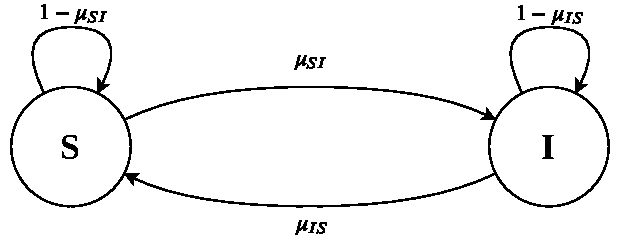
\includegraphics[width=\linewidth]{../img/SIS_model.pdf}
    \caption{SIS model representation.}
    \label{fig:sis}
\end{figure}

To simulate this we do like in SIR but, at each time step, we go through all nodes of the network and do the following:
\begin{itemize}
    \item \textbf{If node i is Susceptible:} 
    \begin{itemize}
        \item[] $n=\sum_{j\in I}W_i,j$
        \item[] $\mu_{SI}=1-(1-\beta)^n$
        \item[] if $\mu_{SI}>real\_random(0,1)$: i is Infected
        \item[] else: i stays Susceptible  
    \end{itemize}
    \item \textbf{If node i is Infected:} 
    \begin{itemize}
        \item[] if $\gamma>real\_random(0,1)$: i is Recovered
        \item[] else: i stays Infected
    \end{itemize}
\end{itemize}
\subsection{Experiments}
\label{ssec:experiments}